\documentclass[tikz,border=2pt]{standalone}
\usepackage{amsmath,amssymb}
\usepackage{tikz}
\usetikzlibrary{matrix,arrows.meta}

\begin{document}
% Minimum-ratio test for the entering variable x_s: divide each right-hand side by the
% positive coefficient in the pivot column; the smallest ratio (40, row s_3) names the leaving
% variable and the pivot element.
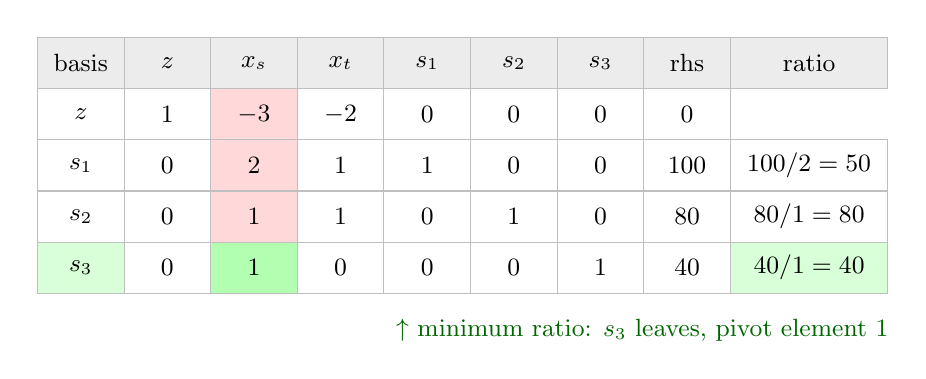
\begin{tikzpicture}[every node/.style={font=\small}, >={Latex[length=1.8mm]}]
	\matrix (T) [matrix of math nodes, nodes={minimum width=1.1cm, minimum height=6.5mm, anchor=center, draw=gray!50}, column 9/.style={nodes={minimum width=2.0cm}}, column sep=-\pgflinewidth, row sep=-\pgflinewidth] at (0,0) {
		|[fill=gray!15]| \text{basis} & |[fill=gray!15]| z & |[fill=gray!15]| x_s & |[fill=gray!15]| x_t & |[fill=gray!15]| s_1 & |[fill=gray!15]| s_2 & |[fill=gray!15]| s_3 & |[fill=gray!15]| \text{rhs} & |[fill=gray!15]| \text{ratio} \\
		z & 1 & |[fill=red!15]| -3 & -2 & 0 & 0 & 0 & 0 & \\
		s_1 & 0 & |[fill=red!15]| 2 & 1 & 1 & 0 & 0 & 100 & 100/2=50 \\
		s_2 & 0 & |[fill=red!15]| 1 & 1 & 0 & 1 & 0 & 80 & 80/1=80 \\
		|[fill=green!15]| s_3 & 0 & |[fill=green!30]| 1 & 0 & 0 & 0 & 1 & 40 & |[fill=green!15]| 40/1=40 \\
	};
	\node[green!40!black, anchor=north east] at ([yshift=-2pt]T.south east) {$\uparrow$ minimum ratio: $s_3$ leaves, pivot element $1$};
	\end{tikzpicture}
\end{document}
